\section{Arsitektur Sistem Operasi Linux}
\subsection{Kernel}
	Kernel Linux merupakan kernel yang digunakan dalam sistem operasi GNU/Linux. Kernel ini merupakan turunan dari sistem operasi UNIX, yang mana di rilis menggunakan lisensi GNU \textit{General Public License} (GPL) dan dikembangkan oleh programmer di selururh dunia karena sifatnya yang \textit{open source}. Kernel ini merupakan inti dari sistem operasi komputer dengan memiliki kontrol penuh atas segala dalam sistem tersebut. Kernel ini menghubungkan antara perangkat lunak dan perangkat keras seperti pada gambar \textbf{\ref{kernel}}, salah satu program pertama yang memuat fungsi kernel ini yaitu dimuat didalam start-up setelah proses bootloader.

\begin{figure}[!htbp]
\centerline{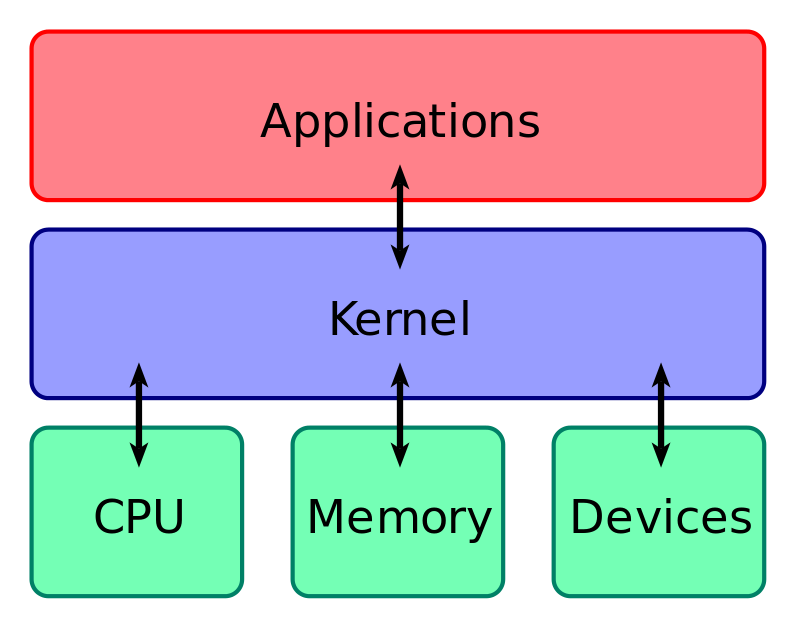
\includegraphics[width=0.75\textwidth]{Figures/Kernel_Layout.png}}
\caption{Kernel connect}
\label{kernel}
\end{figure}

\lstinputlisting[caption=contoh dasar kode program kerne membuat hello world,label={lst:kode dasar}]{src/contoh.tex}

\subsection{struktur data kernel}
	Ketika kernel melakukan sebuah proses, data-data proses tersebut akan disimpan secara periodik ke dalam bentuk file-file. Untuk dapat melihat data kernel, maka file-file tersebut harus diparsing setiap saat dikarenakan datanya yang dinamis \cite{raharja2001pengenalan}. Cara termudah untuk melakukan hal tersebut yaitu menggunakan perintah \textbf{cat} \ref{lst:kode dasar2}

\lstinputlisting[caption=Perintah cat pada linux,label={lst:kode dasar2}]{src/cat.sh}
File-file ini akan tersimpan di dalam direktori yang tersetruktur dalam direktori /proc.